\subsection{Anwendung}\label{sec:anwendung}

Um einen lückenlosen Betrieb zu gewährleisten, ist ein Ablauf für den Gebrauch des Dojos notwendig. Dieser Ablauf kann zusammenfassend in vier Schritte unterteilt werden und ist nachfolgend in Abbildung \ref{fig:Anwendungsablauf Dojo} ersichtlich.

\begin{figure}[H]
	\begin{center}
		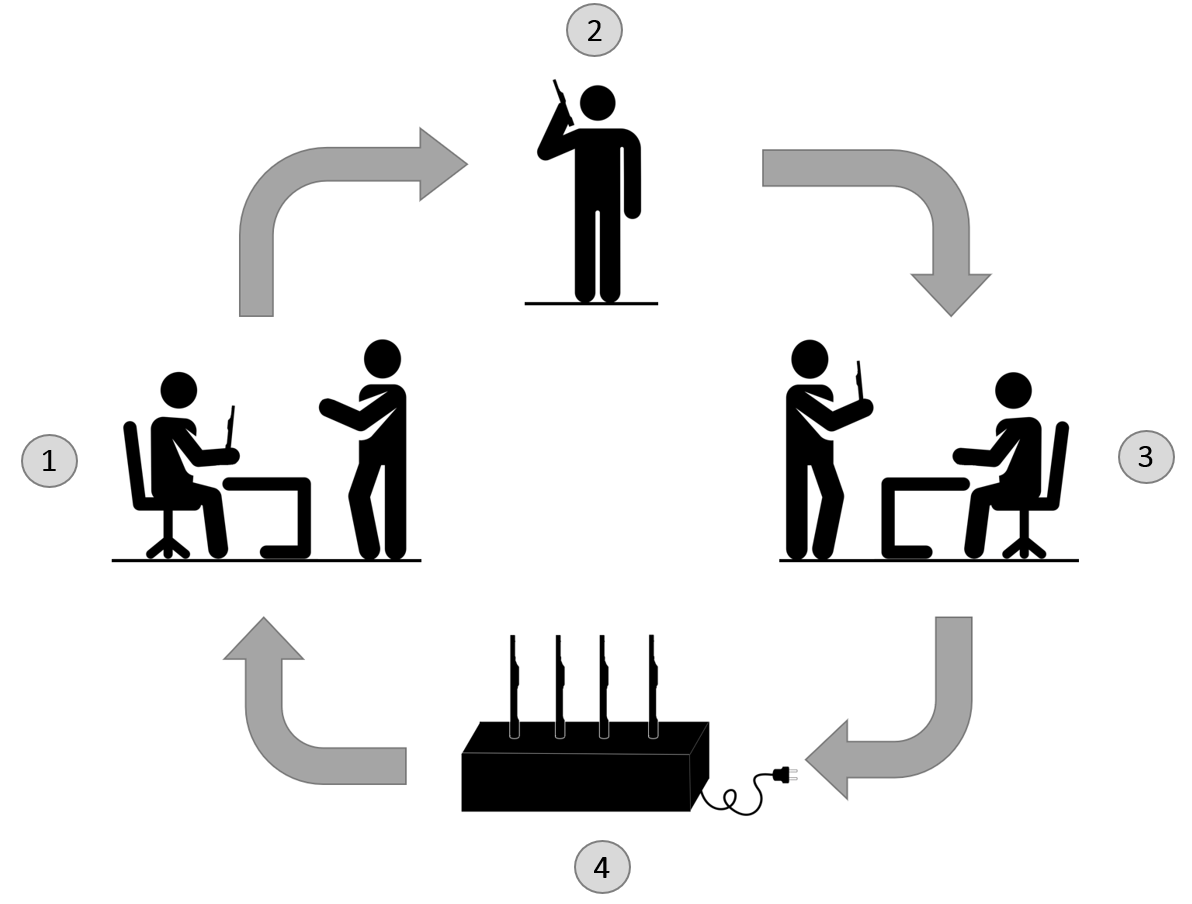
\includegraphics[width=140mm]{data/Ladezyklus.png}
		\caption[Anwendungsablauf des Dojos]{Anwendungsablauf} %picture caption
		\label{fig:Anwendungsablauf Dojo}
	\end{center}
\end{figure}

Der erste Schritt beinhaltet die Dojo Ausgabe beim Empfang. Hierbei wird festgelegt zu welchen Bereichen der Besucher Zutritt erhalten soll. Dies ist abhängig von den Wünschen des Besuchers. Die Auswahl der Sprache wird nachfolgend im Abschnitt \nameref{sec:sprachauswahl} beschrieben. Zu beachten gilt es, dass jeweils die Geräte ausgegeben werden, welche sich am längsten in der Ladestation (Schritt 4) befinden. Hierbei hilft eine Signal-LED am Dojo, welche den Ladestatus gemäss definiertem Farbschema ausgibt. Ein lückenloser Betrieb wird erreicht, wenn die Stückzahl der Audio-Guide Geräte in etwa der Anzahl der Besucher pro Tag entspricht.
\\
\\
In Schritt 2 befindet sich der Besucher auf dem Rundgang mit dem Dojo als Audio-Guide. Der Nutzer hat hierbei die Möglichkeit während dem Rundgang Bilder zu \glqq liken\grqq . Weitere Funktionen und die Bedienung des Dojos selber, ist im vorherigen Unterkapitel \ref{sec:funktionsweise} beschrieben.
\\
\\
Die Abgabe erfolgt in Schritt 3. Hier hat der Besucher die Möglichkeit \glqq gelikte\grqq Bilder als Broschüre zu erhalten oder diese per Mail zu erhalten. Das entgegengenommene Dojo kann für den nächsten Besucher gereinigt werden.
\\
\\
Sobald das Dojo entgegengenommen wurde und alle benötigten Informationen (\glqq likes\grqq) extrahiert wurden, wird es wie in Schritt 4 ersichtlich aufgeladen. Hierfür ist eine induktive Ladestation notwendig, wobei es die Dojos lediglich in die dafür vorgesehenen Ladebuchsen zustecken gilt. Zur Signalisation des Ladevorganges dient eine in jedem Gerät eingebaute Signal-LED, welche bei Spannungsversorgung zu leuchten beginnt.
\\
\\
\subsubsection*{Sprachauswahl} \label{sec:sprachauswahl}

Die Sprachauswahl wird durch den Besucher selbst eingestellt. Hierbei stehen ihm vier Bluetooth-Beacons zur Verfügung zu welchen er sein Dojo hinhalten kann. Die gewünschte Sprache ist hierbei durch die Landesflagge gekennzeichnet. Ein Beispiel einer solchen Anwendung ist nachfolgend in Abbildung \ref{fig:SprachauswahlBeacon} ersichtlich.

\begin{figure}[H]
	\begin{center}
		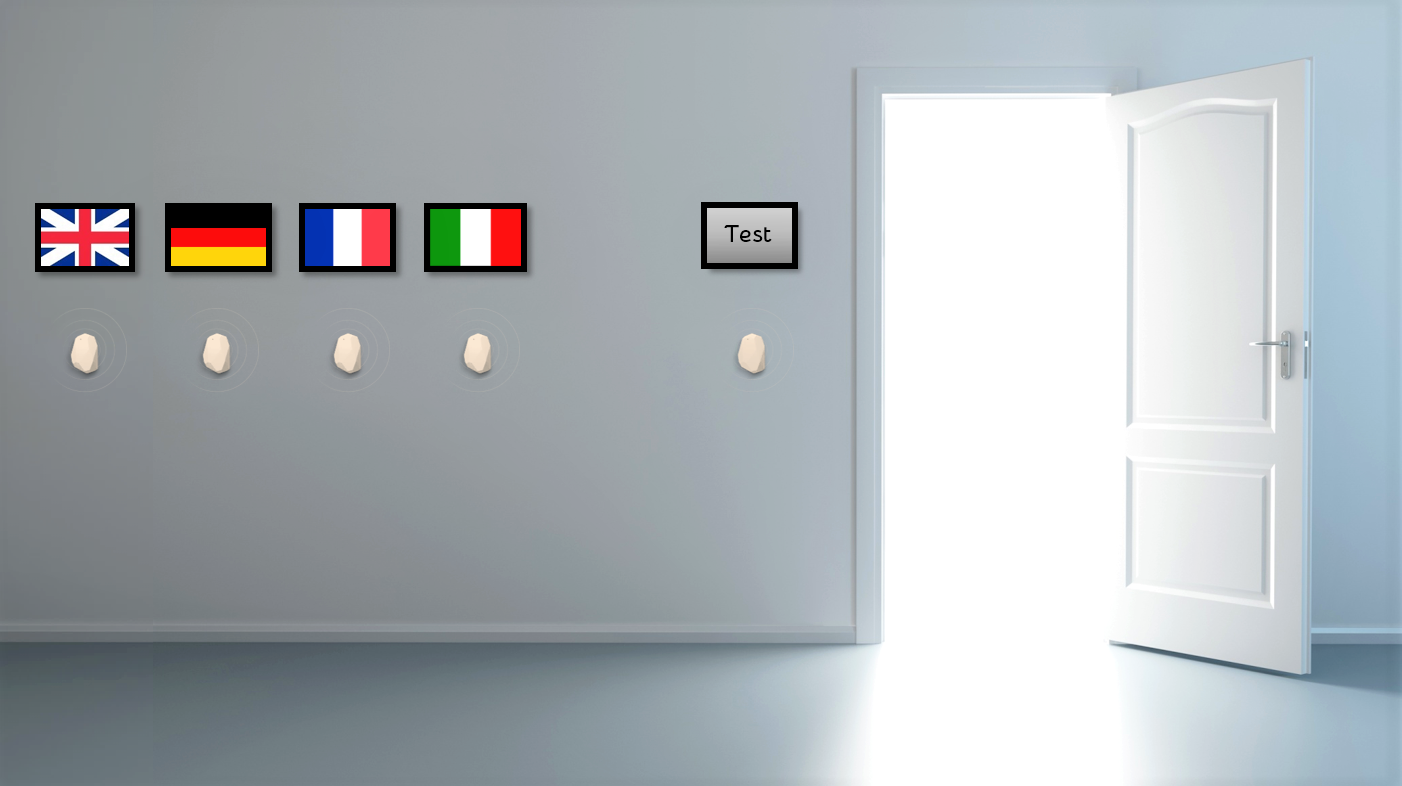
\includegraphics[width=140mm]{data/BeaconSpracherkennung.png}
		\caption[Sprachauswahl mittels Bluetooth-Beacon]{Sprachauswahl mittels Bluetooth-Beacon} %picture caption
		\label{fig:SprachauswahlBeacon}
	\end{center}
\end{figure}

Es ist ersichtlich, dass eine Auswahl aus vier Sprachen möglich ist. Um die gewünschte Sprache auf dem Gerät zu aktivieren, muss der Dojo an den jeweiligen Sprachbeacon heran gehalten werden und gleichzeitig die Playtaste gedrückt werden. Wurde die Sprache erfolgreich ausgewählt, wird ein kurzes Audio-Sample mit der gewählten Sprache abgespielt. Diese kurze Sprachausgabe ist lediglich für die Gewissheit des Besuchers ob die richtige Sprache ausgewählt wurde. Sobald die gewünschte Sprache geladen und getestet wurde, kann der Museumsbesuch gestartet werden.
